\documentclass[journal]{../IEEEtran}

\usepackage{graphicx}
\usepackage{fancyhdr}
\usepackage{epsfig} % for postscript graphics files
\usepackage{graphics} % for pdf, bitmapped graphics files

\pagestyle{fancy}
\lhead{CPE 470/670}
\rhead{\thepage}
\chead{Team 6: Lab 6 Report}
\lfoot{}
\rfoot{}
\cfoot{}

\begin{document}

\begin{titlepage}
    \vspace*{\fill}
    \begin{center}
      {\LARGE \bf Lab 6: Ball Sorting Contest}

      {Team 6: Alexander  C. Woods and Taylor Mansfield}

      November 5, 2014
    \end{center}
    \vspace*{\fill}
  \end{titlepage}


\section{Hardware and Software Design}\label{S.design}
\IEEEPARstart{L}{ine} following is a classic robotics problem

%\begin{figure}[ht]
%\centering
% 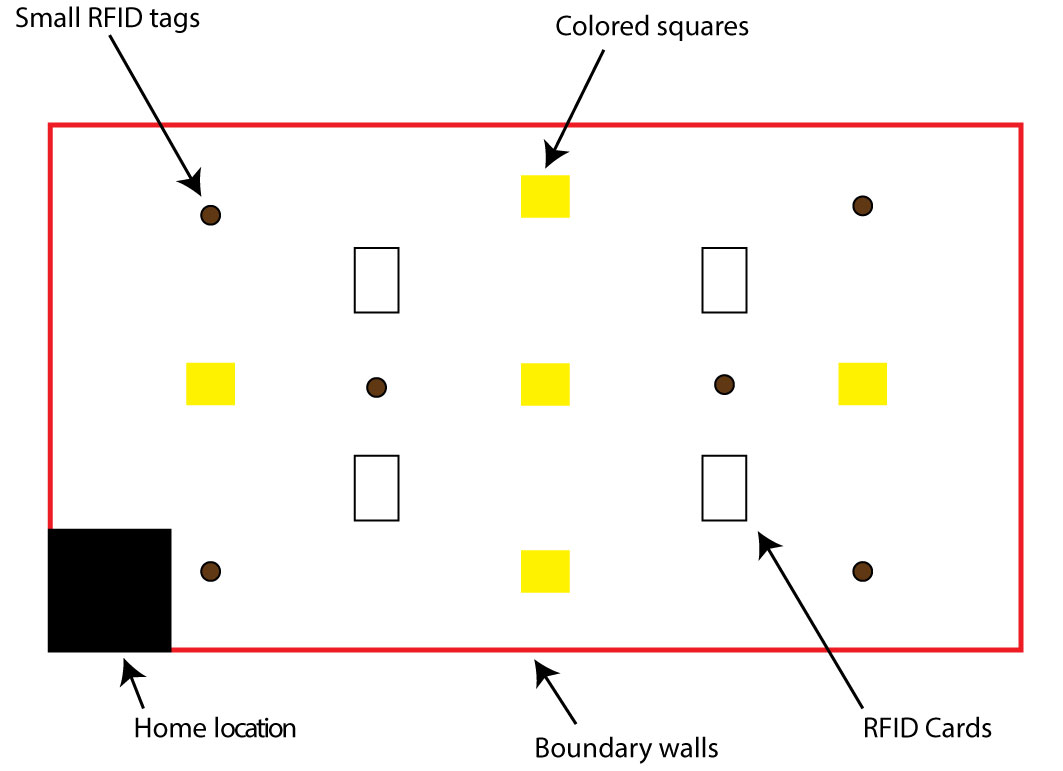
\includegraphics[width=1\columnwidth]{field.jpg}\\
%\caption{The test field is rectangular, with a solid black line for the robot to follow. The end of the black line is marked by a solid yellow square. The home location is designated by the solid black square in the lower left corner.}
%\label{F.field}
%\end{figure}

The hardware required for this challenge

The software design for this challenge 

\begin{equation}\label{E.motor_speed}
    P_{motor} = \frac{P_{max}-P_{min}}{I_{max}-I_{min}}I_{sensor} + offset
\end{equation}

\section{Problems Encountered}\label{S.problems}


\section{Solutions}\label{S.solutions}


\section{Unsolved Problems}\label{S.unsolved}


\end{document}
